
% ------------------------------------------------------------
% ------------------------------------------------------------

\section[Geographical Plots]{Geographical Plots}
%%%%%%%%%%%%%%%%%%%%%%%%%%%%%%%%%%%%%
\subsection{Maps}
%%%%%%%%%%%%%%%%%%%%%%%%%%%%%%%%%%%%%

\begin{frame}[fragile]
\frametitle{Geographic Maps}
  \framesubtitle{Map of Fiji Earthquakes Since 1964}

To overlay a map to a plot containing latitude and longitude, load the package \ttfamily maps: \normalfont 
    \begin{columns}
      \column{0.55\textwidth}
\begin{lstlisting}[ basicstyle=\footnotesize]
data(quakes)
library(maps)
plot(
	quakes$long, 
	quakes$lat, 
	xlim=c(100, 190), 
	ylim=c(-40, 0)
	)
map("world", add=TRUE)
\end{lstlisting}

     \column{0.45\textwidth}
       \begin{center}
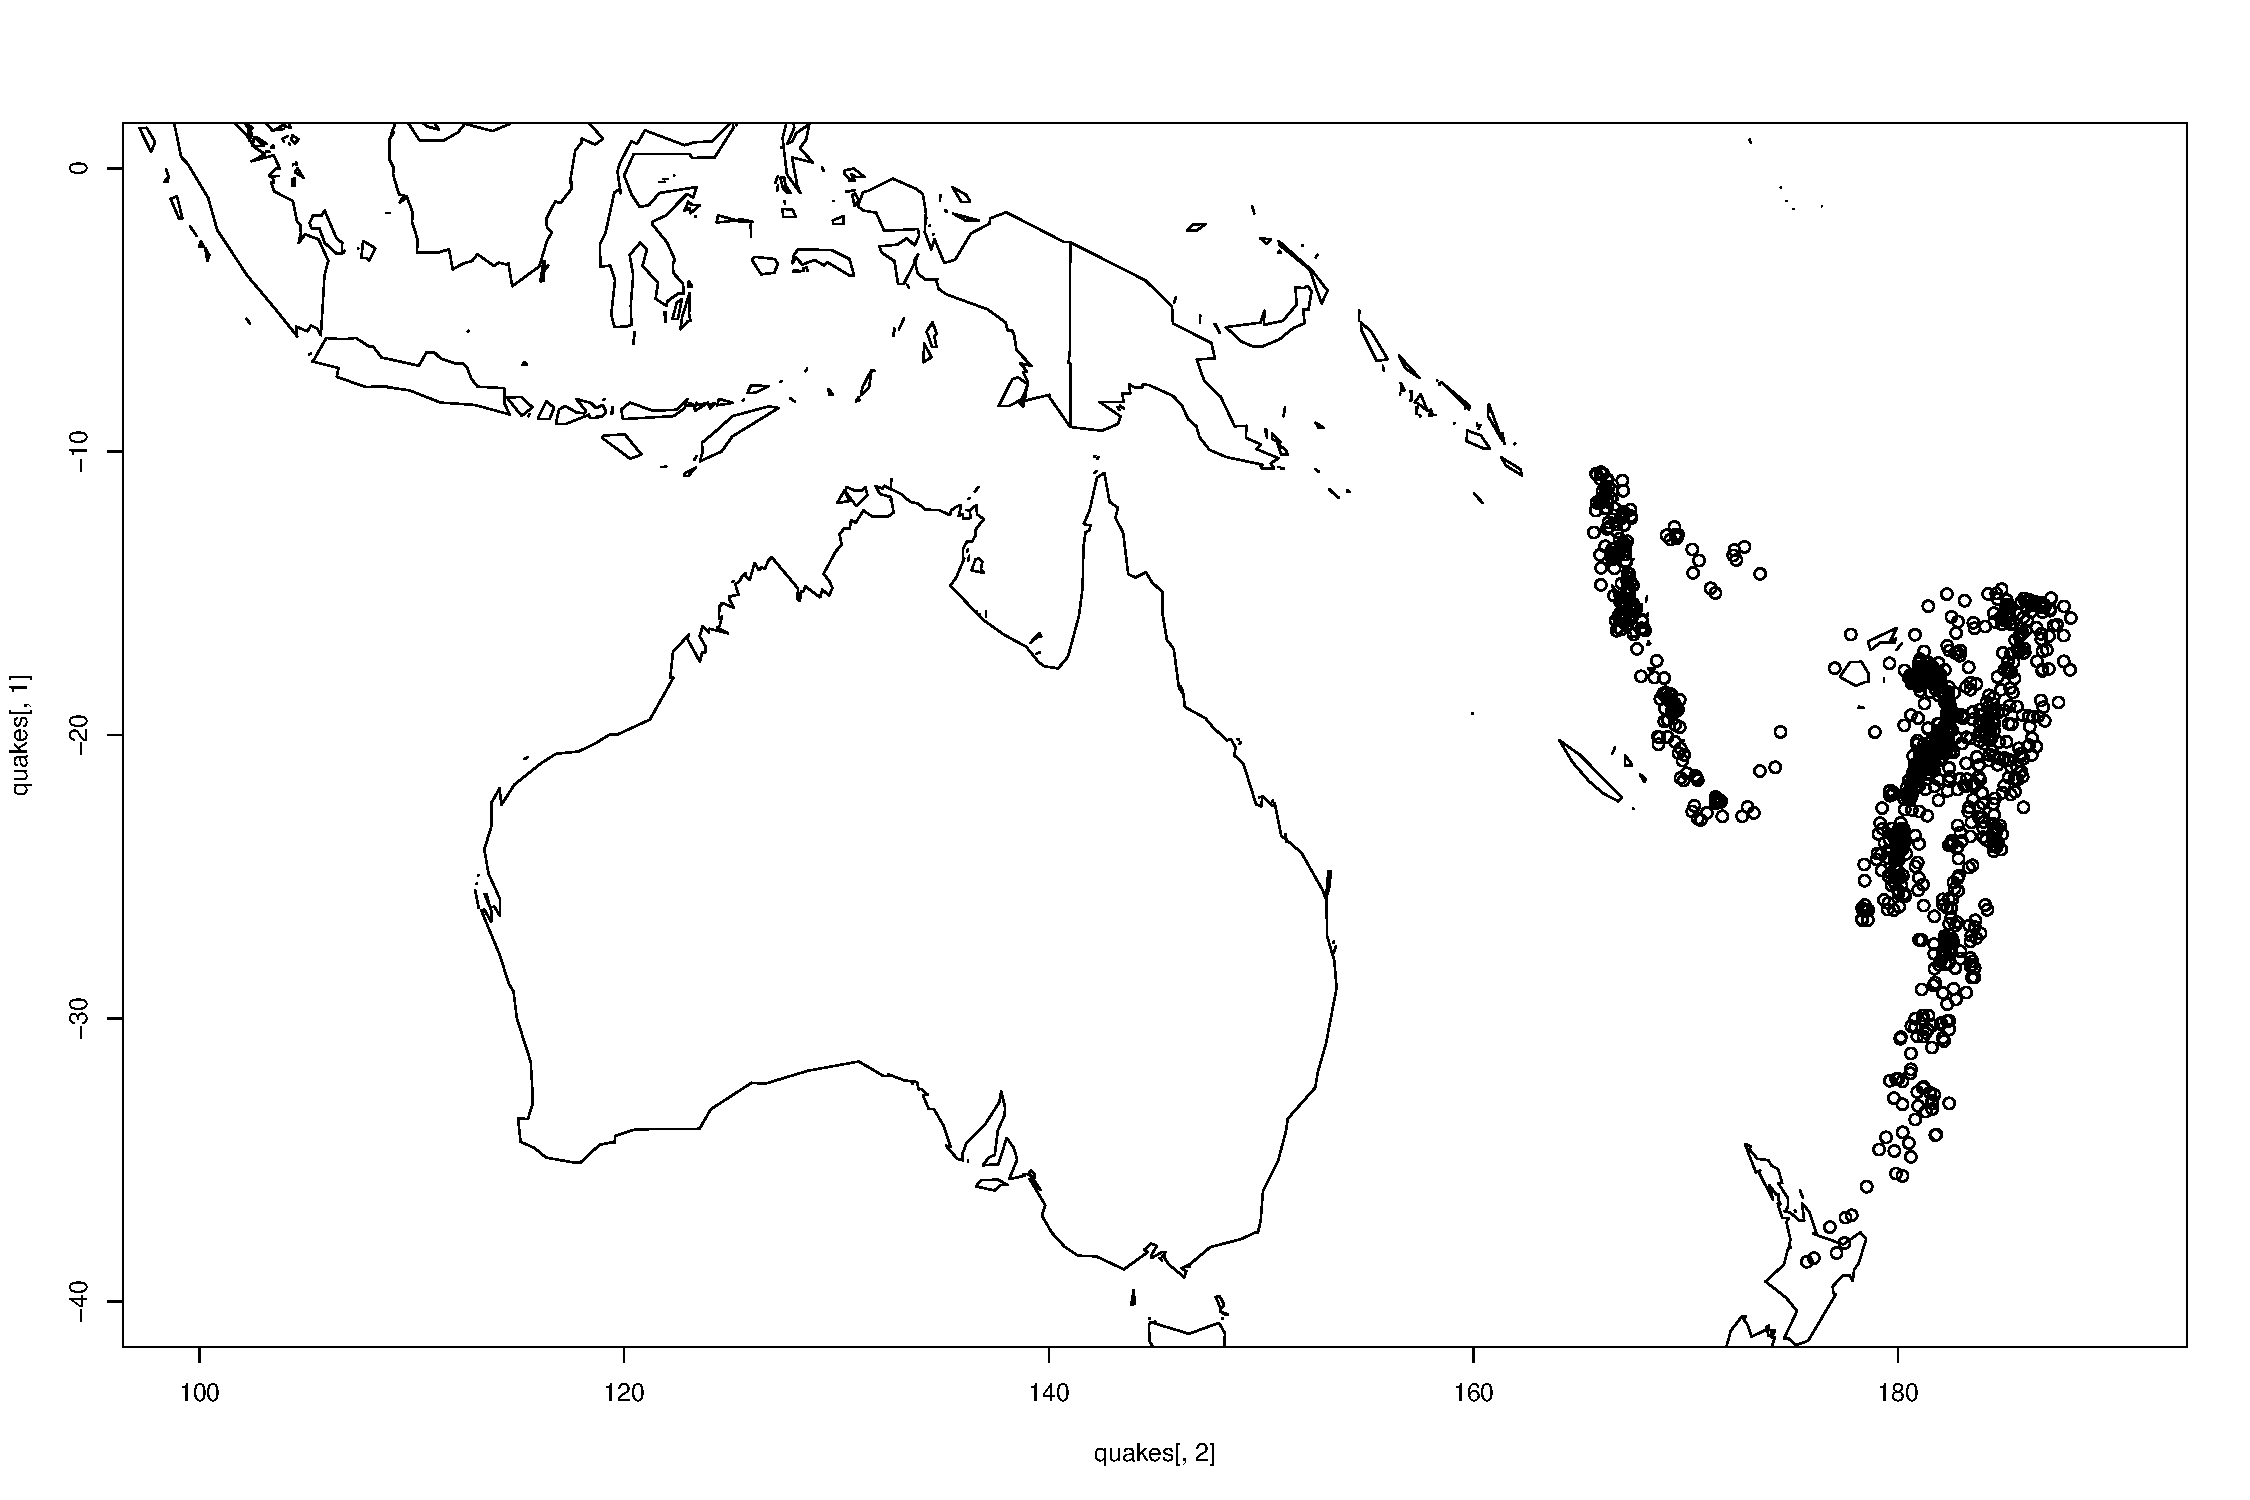
\includegraphics[width = 55mm]{images/Fuji.pdf}
\end{center}
\end{columns}
\end{frame}

%___________
\begin{frame}[fragile, allowframebreaks]
\frametitle{Geographic Maps}
  \framesubtitle{Map of Fiji Earthquakes Since 1964}

To include information on magnitude of earthquake, use \ttfamily cex \normalfont argument of the \ttfamily plot() \normalfont function:
\begin{lstlisting}
# Step 1: Recode magnitude to have 3 categories only
ind<-which(quakes$mag<5)
ind2<-which(quakes$mag<6 & quakes$mag >=5)
ind3<-which(quakes$mag>=6)
color<-rep(NA, length(quakes$mag))
color[ind]<-1; color[ind2]<-2; color[ind3]<-3




# Step 2: Plot
plot(quakes$long, quakes$lat, cex=color, pch=19, col=color, xlim=c(100, 190), ylim=c(-40,0), xlab="Longitude", ylab="Latitude")
legend("topright", pch=19, col=1:3, c("Mag<5", "5<=Mag<6", "Mag>6"), pt.cex=1:3)
map("world", add=TRUE)
\end{lstlisting}

\newpage
       \begin{center}
		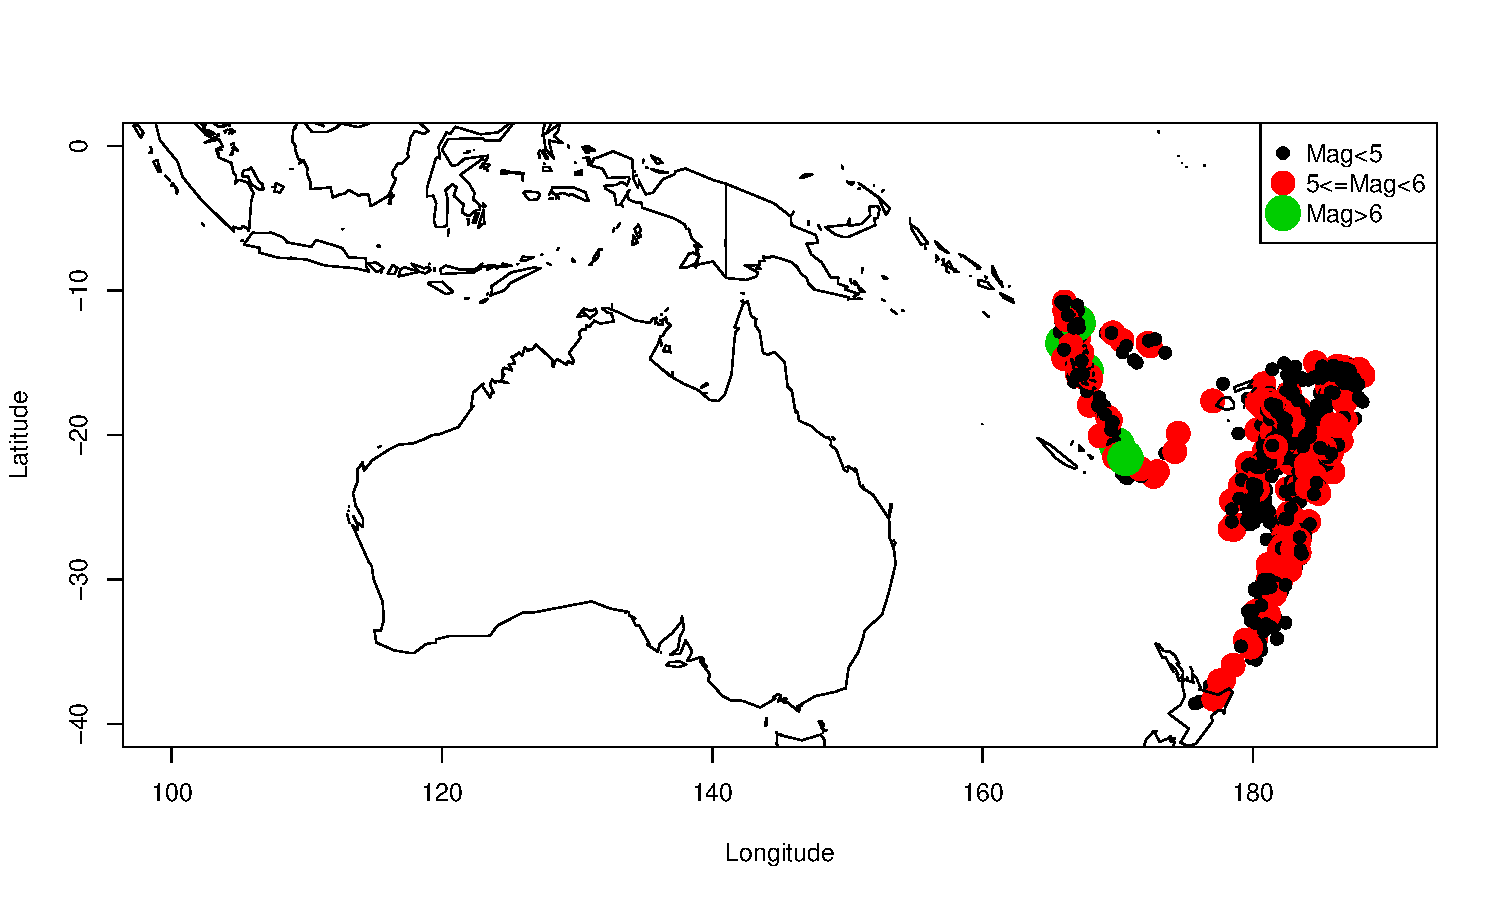
\includegraphics[scale=0.42]{images/fujiColor.pdf}
	\end{center}

\end{frame}


%%%%%%%%%%%%%%%%%%%%%%%%%%%%%%%%%%%%%
\subsection{Projection Maps}
%%%%%%%%%%%%%%%%%%%%%%%%%%%%%%%%%%%%%

\begin{frame}[allowframebreaks, fragile]
\frametitle{Projection Maps}
  \framesubtitle{Map of Fiji Earthquakes Since 1964}

For a different perspective of a map, use  \ttfamily mapproject(): \normalfont 

\begin{lstlisting}
library(mapproj)
library(maps)
m <- map('world',plot=FALSE)
# Projection is Azimuthal with equal-area
map('world',proj='azequalarea',orient=c(longitude=0,latitude=180,rotation=0))
map.grid(m,col=2)
points(mapproject(list(                       y=quakes$lat[which(quakes$mag>=6)],       x=quakes$long[which(quakes$mag>=6)])),    col="blue",pch="x",cex=2)
\end{lstlisting}

\newpage
       \begin{center}
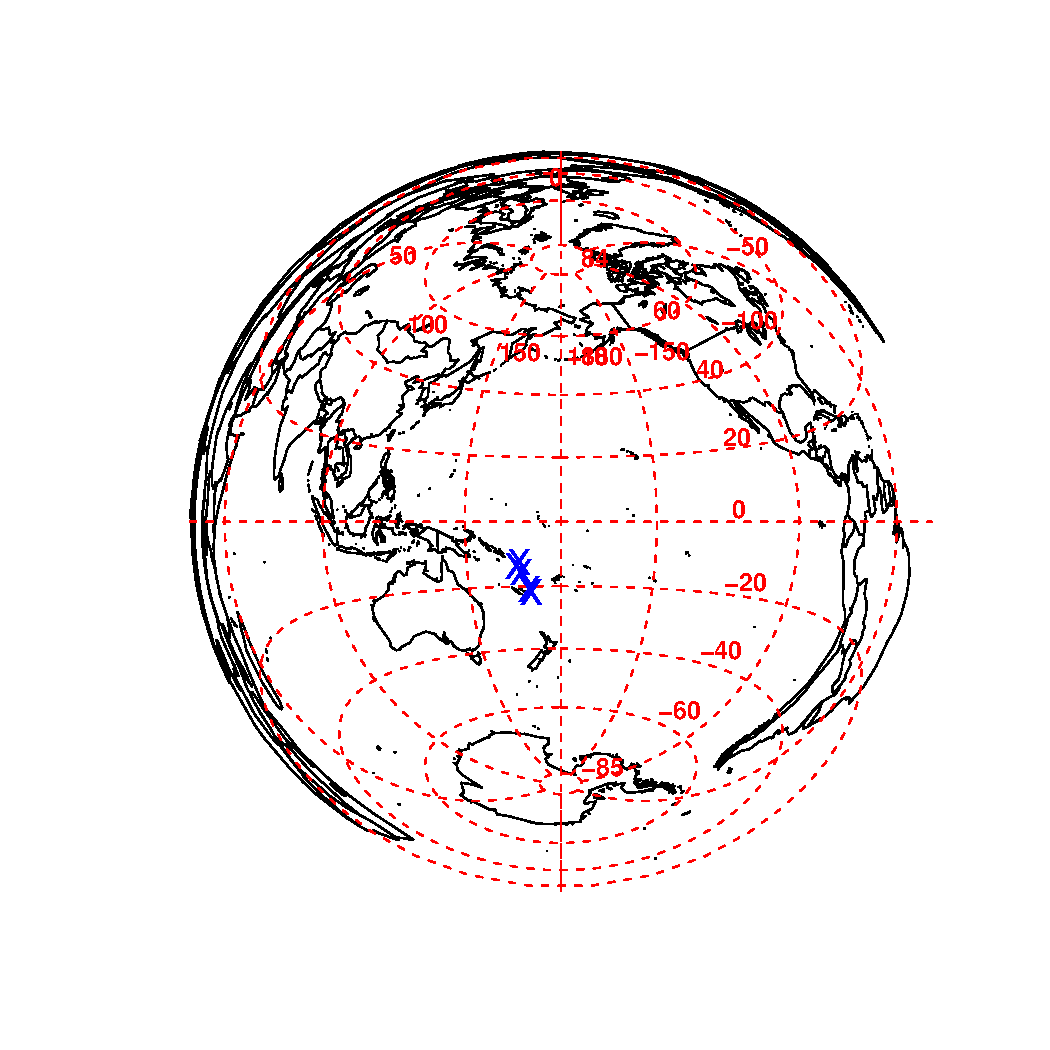
\includegraphics[width = 70mm]{images/Fuji2.pdf}
\end{center}

\end{frame}

% %%%%%%%%%%%
% \begin{frame}[fragile]
% 	\begin{alertblock}{Bonus Feature of the \ttfamily maps \normalfont package:}
% 		To determine in which part of the world the observations are (based on latitude and longitude), use \ttfamily map.where(): \normalfont
% 			\begin{lstlisting}		
% 				in.what.country<-map.where(database="world", quakes$long, quakes$lat)
% 			\end{lstlisting}
% 		To determine which observations are in the ocean: \normalfont
% 			\begin{lstlisting}
% 				# Number of points in ocean after filtering:
% 				ind<-sum(is.na(in.what.country)); ind
% 				# Number of observations: 1000
% 				# Number in Ocean: 993
% 			\end{lstlisting}
% 	\end{alertblock}

% \end{frame}

% ------------------------------------------------------------
% ------------------------------------------------------------
\subsection{Exercise III}
\begin{frame}
	\frametitle{Exercise III}
	For the \ttfamily ozone \normalfont data set \footnote{\ttfamily http://www.ats.ucla.edu/stat/R/faq/ozone.csv\normalfont}, determine the region of the world that the observations correspond to and overlay the appropriate map.
\end{frame}
%ozone<-read.table("http://www.ats.ucla.edu/stat/R/faq/ozone.csv", sep=",", header=T)
%attach(ozone)
%plot(Lat~Lon, xlim=c(-125, -113), ylim=c(31,42))
%map("state", "california", add=TRUE)